\documentclass[draft=false
              ,paper=a4
              ,twoside=false
              ,fontsize=11pt
              ,headsepline
              ,BCOR10mm
              ,DIV11
              ]{scrbook}
\usepackage[ngerman,english]{babel}
%% see http://www.tex.ac.uk/cgi-bin/texfaq2html?label=uselmfonts
\usepackage[T1]{fontenc}
%\usepackage[utf8]{inputenc}
\usepackage[latin1]{inputenc}
\usepackage{libertine}
\usepackage{pifont}
\usepackage{microtype}
\usepackage{textcomp}
\usepackage[german,refpage]{nomencl}
\usepackage{setspace}
\usepackage{makeidx}
\usepackage{listings}
%\usepackage{natbib}
\usepackage[ngerman,colorlinks=true]{hyperref}
\usepackage{soul}
\usepackage{hawstyle}
\usepackage{lipsum} %% for sample text
\usepackage{chngcntr}

%% define some colors
\colorlet{BackgroundColor}{gray!20}
\colorlet{KeywordColor}{blue}
\colorlet{CommentColor}{black!60}
%% for tables
\colorlet{HeadColor}{gray!60}
\colorlet{Color1}{blue!10}
\colorlet{Color2}{white}

%% configure colors
\HAWifprinter{
  \colorlet{BackgroundColor}{gray!20}
  \colorlet{KeywordColor}{black}
  \colorlet{CommentColor}{gray}
  % for tables
  \colorlet{HeadColor}{gray!60}
  \colorlet{Color1}{gray!40}
  \colorlet{Color2}{white}
}{}
\lstset{%
  numbers=left,
  numberstyle=\tiny,
  stepnumber=1,
  numbersep=5pt,
  basicstyle=\ttfamily\small,
  keywordstyle=\color{KeywordColor}\bfseries,
  identifierstyle=\color{black},
  commentstyle=\color{CommentColor},
  backgroundcolor=\color{BackgroundColor},
  captionpos=b,
  fontadjust=true
}
\lstset{escapeinside={(*@}{@*)}, % used to enter latex code inside listings
        morekeywords={uint32_t, int32_t}
}
\ifpdfoutput{
  \hypersetup{bookmarksopen=false,bookmarksnumbered,linktocpage}
}{}

%% more fancy C++
\DeclareRobustCommand{\cxx}{C\raisebox{0.25ex}{{\scriptsize +\kern-0.25ex +}}}

\clubpenalty=10000
\widowpenalty=10000
\displaywidowpenalty=10000

% unknown hyphenations
\hyphenation{
}

% MAKE SECTIONS AS CHAPTERS
\renewcommand{\thesection}{\arabic{section}}
\makeatletter
\let\l@section\l@chapter
\makeatother

% FIX FIGURE NUMBERING
\counterwithin{figure}{section}

%% recalculate text area
\typearea[current]{last}

\makeindex
\makenomenclature

\begin{document}
%\selectlanguage{ngerman}

%%%%%
%% customize (see readme.pdf for supported values)
\HAWThesisProperties{Author={Lotte Steenbrink}
                    ,Title={Ausarbeitung}
                    ,EnglishTitle={Routing in the Internet of Things}
                    ,ThesisType={Routing in the Internet of Things}
                    %,ExaminationType={Bachelorpr�fung}
                    %,DegreeProgramme={Master of Science Angewandte Informatik}
                    %,ThesisExperts={Prof. Dr. Erstpr�fer \and Prof. Dr. Zweitpr�fer}
                    ,ReleaseDate={\today}
                  }

%% title
\frontmatter
%% output title page
\maketitle

\onehalfspacing

%% add abstract pages
%% note: this is one command on multiple lines
%\HAWAbstractPage
%% German abstract

% TODO!!!
%{Routing, 6LowPAN, IoT, MANET, LLN, DTN}%
%{Dieses Dokument \ldots}
%% English abstract
%{keyword 1, keyword 2}%
%{This document \ldots}

\newpage
\singlespacing

\tableofcontents
\newpage
%% enable if these lists should be shown on their own page
%%\listoftables
\listoffigures
%\lstlistoflistings
\newpage

\newpage
\chapter*{Glossary}
\printglossaries
\newpage

% make little page headers display section titles
\newcommand{\currentsection}{}
\let\oldsection\section
\renewcommand{\section}[1]{\oldsection{#1}\renewcommand{\currentsection}{#1}}
\ihead{\currentsection}

%% main
\mainmatter

\onehalfspacing

\section{Introduction}
\label{sec:introduction}
%==============================================================================
With vast technological advancements and the growing popularity of digital assistance in everyday life and work environments that goes along with it, technologies are needed to evolve these application domains to the next level. One vision for this is the \gls{IoT}: interconnected devices, embedded in all kinds of objects. In order to turn this vision into reality, routing protocols are needed to aid the communication between these \emph{things} in a decentralized, self-organized and changing infrastructure.

\subsection{The Internet of Things}
\label{subsec:intro_IoT}
%==============================================================================
The \gls{IoT} is the vision of machine-to-machine communication between devices embedded in
things, so-called \emph{smart objects} \cite{KULeuven-314567}.
To avoid interference with the usability of the \emph{thing}, IoT devices are small, embedded devices, equipped with only a few hundred kB of ROM. They are powered by batteries, which have to last for months or even years without maintenance.\\
%TODO: application areas (examples)
IoT devices are organized in a mesh network which is connected to the Internet through a gateway router. This sets them apart from traditional \glspl{WSN}.
Traffic is usually connectionless and sparse, with small payloads. The traffic patterns emerging from IoT devices vary with the application area: Building Automation, as described by \cite{RFC5867}, commonly generates point-to-point-traffic, while centralized Home Automation applications of \cite{RFC-5826} exhibit a mixture of multipoint-to point and point-to-multipoint traffic.
Because interference with foreign signals, fading connectivity, and signal reflection or scattering are often encountered in wireless mesh networks, there is no guarantee for bidirectional connectivity.

\subsection{The Network Stack}
\label{subsec:networkstack}
%==============================================================================
\begin{figure}[ht!]
  \centering
    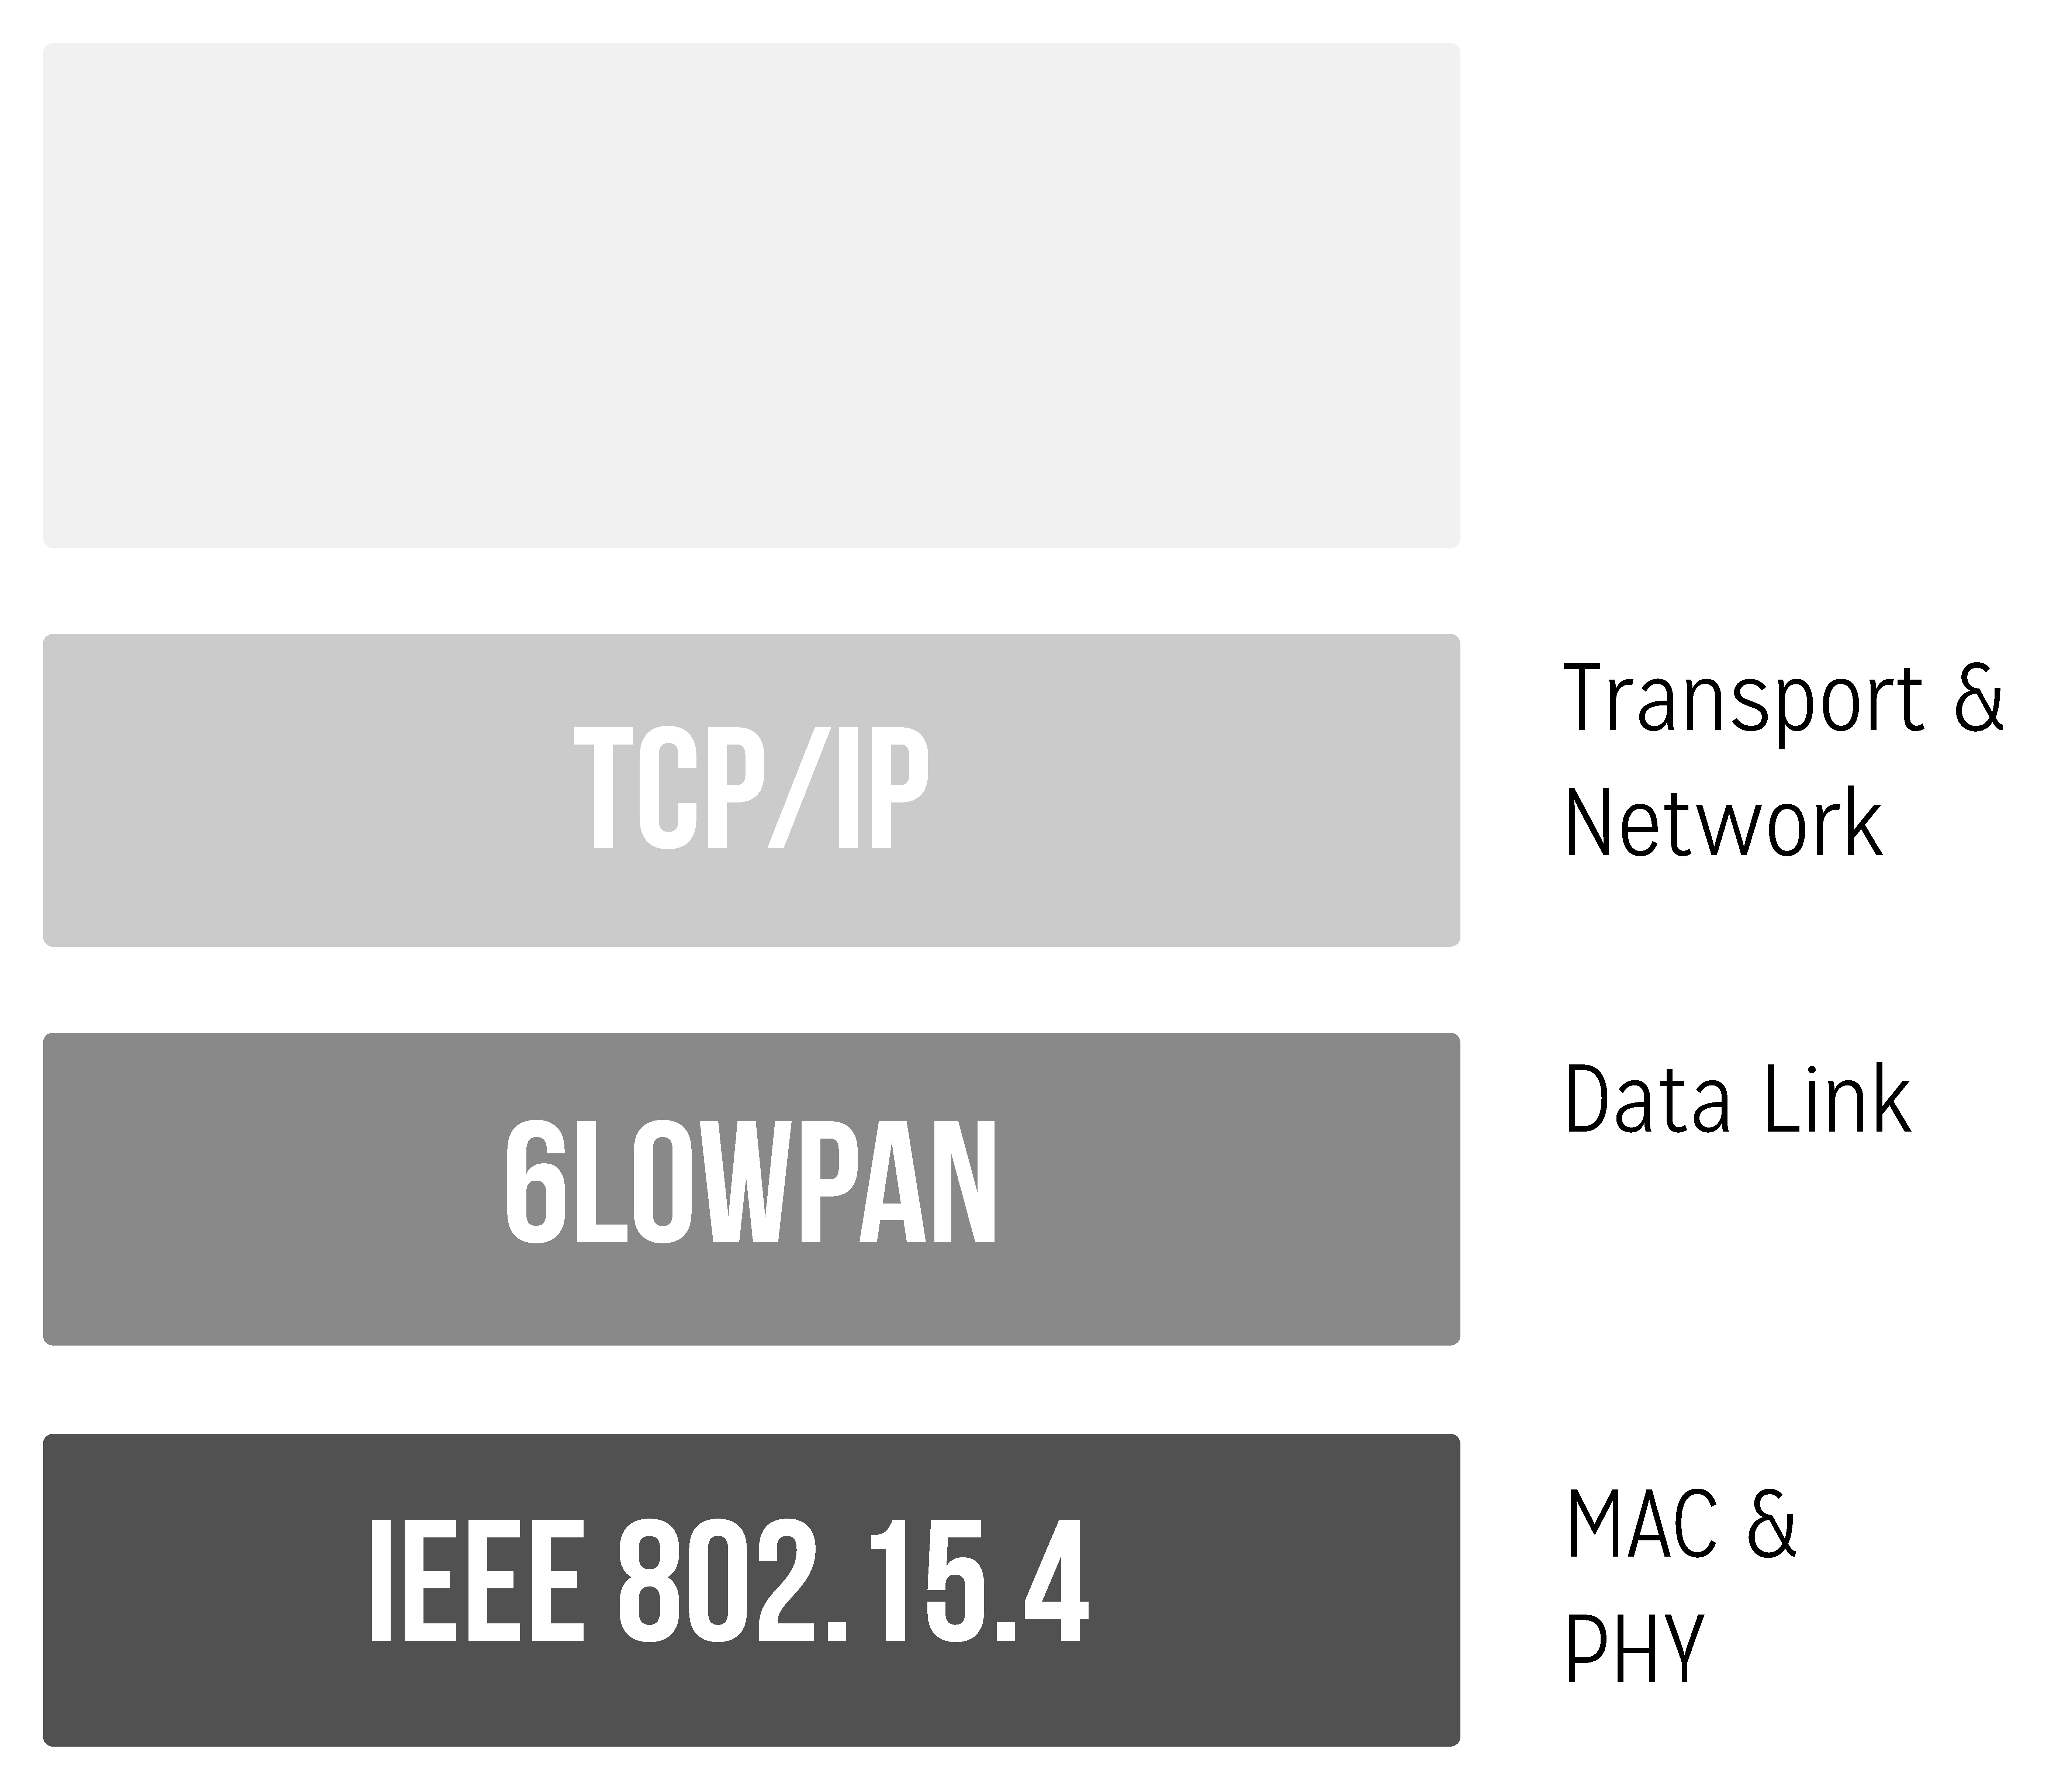
\includegraphics[width=0.9\textwidth]{graphics/networkstack.eps}
  \caption{Comparison of traditional and IoT Network Stacks.}
  \label{fig:networkstack}
\end{figure}

Because the IoT differs from the ``traditional'' Internet in crucial aspects, the use of a custom network stack as illustrated in Fig. \ref{fig:networkstack} is necessary.\\
The IEEE 802.15.4 Data Link and Physical layers have been optimized for energy-efficiency and the ability to be deployed on cheap device. Its \gls{MTU} is a mere 127 bytes. This limitation conflicts with the minimal MTU of 1280 bytes dictated by IPv6, generating the demand for an adaptation layer: 6LoWPAN. Here, IPv6 headers are compressed; packets exceeding the new 127 byte MTU are fragmented. The fragments produced can be reassembled by all border routers connecting a 6LoWPAN network to the Internet.

\subsection{Requirements and key challenges for routing protocols}
\label{subsec:intro_requirements}
%==============================================================================
\cite{RFC-5826}, \cite{RFC5548} and \cite{RFC5867} list requirements for a routing protocol in the differing scenarios of Home Automation, Urban-\glspl{LLN} or Building Automation. Even though these fields may all be categorized as IoT-adjacent, their characteristics differ vastly in terms of traffic flow and patterns, network size, and degree of mobility. %(TODO. lieber nochmal überprüfen)
Despite these differences, the domains of their requirements can be classified into four categories:

\begin{description}
\item{\emph{Traffic Patterns:}} A routing protocol for the IoT has to match the traffic pattern of its area of deployment. Since patterns vary from network to network, as shown in \ref{subsec:intro_IoT}, there is most likely not \emph{one} protocol to rule them all, but rather at least one appropriate protocol for each subdivision of IoT deployments.

\item{\emph{Energy efficiency:}} The deployment of battery-driven nodes running autonomously for extended periods of time is one of the cornerstones of the IoT. A routing protocol that is resourceful in terms of energy consumption is vital to the functionality of an IoT-based network.
Closely tied to these efforts is the topic of energy-\emph{awareness}. A protocol able to communicate its nodes' constraints is able to make more informed routing decisions based on this information.

\item{\emph{Scalability:}} The protocol should scale to a network size ranging from 100 to 1,000,000 nodes, both in terms of performance as well as memory usage: an increase in network size may not lead to an explosion in routing table size.

\item{\emph{Mobility:}} Even though the \gls{IoT} does not typically experience a lot of movement, a suitable routing protocol should be able to cope with sparse location changes of single nodes.
\end{description}
% TODO: was ist mit code image size?
% challenges
In addition to the requirements listed above, the nature of the \gls{IoT} poses unique challenges to any routing protocol serving them.

\begin{description}
\item{\emph{Bidirectionality:}} As with all wireless networks, bidirectional connectivity between links is not guaranteed. %Even moreso in \gls{IoT} deployments:
A routing protocol for the \gls{IoT} has to be able to recognize and avoid unidirectional links at the least, and may be able to use them in one direction at best.

\item{\emph{Transmitter usage:}} Concerning energy consumption, the transmitter is the most expensive component of a constrained device.
It is therefor advisable to use it as sparsely as possible. %, letting the device go into deep sleep mode when it is not needed. % TODO: was ist mit wakeup costs?
\end{description}

\subsection{Related research}
\label{subsec:intro_related_fields}
%==============================================================================
Because the \gls{IoT} is a budding field, few research is explicitly tailored to its characteristics.
Nonetheless, adjacent fields have produced work which explores problems which are familiar to the \gls{IoT}, most notably the research fields of \glspl{MANET}, \glspl{DTN} and \glspl{LLN}.
\section{Approaches}
\label{sec:approaches}
%==============================================================================
In order to meet the constraints of the \gls{IoT} as described in section \ref{subsec:intro_requirements}, a routing protocol may employ different strategies. This section lists promising mechanisms and approaches which may form the building blocks if a successful routing protocol for the IoT.

\subsection{Protocol characteristics}
\label{subsec:appr_protocol_characteristics}
%==============================================================================
Each routing protocol exhibits core characteristics which form the very base of its workings.
In the following, characteristics which may be most beneficial in an \gls{IoT} environment will be discussed.

\subsubsection{Proactive vs. Reactive}
\label{subsec:appr_char_reactive}
%...............................................................................
With the exception of hybrid approaches, routing protocols either fall in the category of proactive or reactive.
\begin{description}
\item{\emph{A proactive protocol}} gathers routing information proactively, attempting to have an overview of the entire network's topology at all times. Typically, the periodic distribution of \glspl{beacon} provides nodes with insight about the existence and quality of connection to their neighbors.
This provides for great performance in terms of latency, but can wreak havoc on the battery lifetime: In networks which experience sparse traffic, most of the topology information exchanged can be considered protocol overhead which will drain a device's batteries unnecessarily.
\item{\emph{Reactive protocols}} search for routes on-demand: only when a transmission towards another node is started, the route discovery process (towards this specific node) is triggered. In consequence, topology information is only exchanged when needed, saving energy. The downside to reactive protocols is their latency: because routes are discovered on-demand, transmissions over unknown or expired routes face delays, for which either the application or the routing protocol has to account by buffering or dropping data.
\end{description}

\subsubsection{Hop-by-Hop vs. Source Routing}
\label{subsec:appr_hbh_source}
%...............................................................................
Packet forwarding may be either carried out hop by hop or through source routing. With the former, each router stores a small part of each route it is participating in: the destination of the route, and over which of its neighbors packets towards this destination should be forwarded. With the latter, the entire path of a route is embedded in its packet header. While this has the benefit of memory-efficiency, it increases header sizes and traffic volumes dramatically. Routes may become stale before the packet carrying them in their header has reached its destination. With the relatively small MTU of IEEE 802.15.4 and the moderate mobility in the \gls{IoT}, this makes for an unfortunate combination.

\subsubsection{Information Centric}
\label{subsec:appr_char_infocentric}
%...............................................................................
\glspl{ICN} are not merely a routing protocol, but an entirely new networking paradigm. Oftentimes, it does not matter to the recipient who sends them the data they requested, they are merely interested in receiving the data at all. ICN picks this up: instead of asking single addresses for data, a node will ask the network \cite{ahlgren_ccn_survey}.
%This is especially useful if data is location-dependent, i.e. if it is likely that a node will want to receive information stemming from its surroundings.
Since some \gls{IoT} use cases, like the evaluation of environmental data, are more focused on the information than its origin as well, ICN may be a suitable solution for some IoT deployments.\\
%TODO: explanation: what is the task of a routing protocol?
Because \gls{ICN} was designed with large-scale, cabled networks in mind, it exhibits some characteristics problematic for the deployment in the \gls{IoT}:
%The header overhead it produces may exceed
Connections are assumed to be bidirectional, with no mechanisms to ensure that this assumption holds.\\
With some ICN protocols, all routers cache the data they forward. Considering that memory is very limited on IoT nodes, this may prove to be problematic. Additionally, data which provides an update for a previous information often doesn't update its predecessor, but is stored as a copy, consuming even more storage space \cite{mehlis_ccn_iot}.

\subsection{Mechanisms}
\label{subsec:appr_mechanisms}
%==============================================================================
Routing protocols may be equipped with a myriad of mechanisms influencing the way they make routing decisions. In the following, some mechanisms that may be beneficial to IoT protocols will be highlighted.

\subsubsection{Energy-aware metrics}
\label{subsec:appr_mechanisms_metrics}
%...............................................................................
Metrics are used to quantify the quality of a link or route under certain aspects.
The most commonly deployed metric is Hop Count, with which the route using the fewest hops is chosen. However, this is often less than ideal: not all links are created equal in quality, and long-distance links are especially prone to be lossy.
% TODO: link state vs distance vector -> additive vs ??? metriken beleuchten?
%Problem: energielevel bleibt nicht gleich; metrikinfos muessen evtl oefter ausgetauscht werden? passiert vllt bei OLSR, bei AODV aber definitiv nicht.. was ist mit LOADng?
Energy-awareness may be introduced to existing routing protocols with the help of suitable metrics. A metric which takes energy levels on either the node or network level may influence the routing decisions of a protocol in a way which preserves energy resources.\\
\cite{rfc6551} specify several routing metrics for the \gls{RPL} protocol, some of which may be interesting for other deployments as well. Notable are:\\
\emph{Node Energy:} The energy level of a node may be taken into account in different ways: most intuitively, it may be beneficiary to choose a route over nodes with great residual energy in order to elongate its lifetime and relieve nodes with fewer resources. In doing so, the value of residual energy has to be put into context by the transceiver costs of the individual node as well as its expected lifetime: It may be beneficial to use a node with less battery which is likely to be recharged in the near future (e.g. a mobile device on the nightstand) than one with high residual energy that has to last for a while (e.g. a node in the wall)\footnote{Example as published in \cite{rfc6551}, p. 13}. \\
\emph{Throughput:} When the data sent over a router exceeds the amount of throughput it is able to handle, the resulting packet loss will cause retransmissions, wasting energy on redundant communication. Therefor, a router may specify the throughput it is able to handle.\\
\emph{Latency:} Different types of information may have different latency constraints, for instance because the data may become stale quickly, is important in case of emergency or may trigger timeouts. By taking these requirements into account, a protocol is able to distribute the network load in a way that supports different traffic requirements.\\
These approaches can be combined: \cite{fuzzymetrics} proposes the use fuzzy logic %(TODO: cite fuzzy logic for systems engineering?)
to merge several relevant characteristics of a route or link into one statement about its quality, in this case \emph{number of hops}, \emph{residual energy} and \emph{Received Signal Strength Indicator}.%  (Problem: Paper ist leider sehr vage und versucht, 3 Dinge auf einmal zu zeigen, aber ich mag die Idee...)


\subsubsection{Multipath routing}
\label{subsec:appr_mechanisms_multipath}
%...............................................................................
A protocol employing multipath routing seeks to find and use alternate paths towards every destination. This distributes the cost of forwarding packets among more nodes, saving the energy of individual, highly-frequented nodes. % TODO evtl auch nützlich bei unidiretional nodes? gibts da bestrebungen?
\cite{wsn_survey}

\subsubsection{Probabilistic routing}
\label{subsec:appr_char_probabilistic}
%...............................................................................
With probabilistic routing, routing decisions are calculated based on probabilistic values.\\
The most primitive way to do this is gossiping: Data is flooded through the network like a rumor, but every packet is only forwarded with a probability \emph{p}. This way, traffic overhead is reduced.\\
A more elaborate approach is to predict the chance of delivery towards a certain destination through mobility patterns or previous experience and base forwarding decisions on this prediction.

\section{Protocols}
\label{sec:protocols}
%==============================================================================
In the preceding section, the building blocks of an \gls{IoT} routing protocol, both essential and additional, have been discussed.
This chapter provides an overview over routing protocols that are comprised of these building blocks. Each characteristic presented in section \ref{subsec:appr_protocol_characteristics} is represented by at least one protocol.\\
Each protocol fulfills the criteria listed in section \ref{subsec:criteria} and employs at least one of the approaches described in section \ref{sec:approaches}. The protocols are roughly ordered in accordance with the order from section \ref{sec:approaches}.
Not all of the protocols presented have been designed with the IoT in mind; most stem from adjacent fields of research such as \glspl{DTN} or \glspl{MANET}. %TODO. woher kommt icn zeug?
Despite this, they exhibit characteristics which may make them suitable for the \gls{IoT}.

\subsection{Criteria}
\label{subsec:criteria}
%==============================================================================
During the past 15 years, an overwhelming amount of routing protocols and protocol modifications for \glspl{LLN} and \glspl{MANET} have been published. To sieve through these contributions, a set of criteria has been created and applied to all candidate protocols.
\begin{description}
\item{\emph{Suitability for the IoT:}} A routing protocol has to apply to at least one topology and traffic flow scenario common in the \gls{IoT}. It should be scalable to a certain extent, and be able to cope with unidirectional routes.
\item{\emph{Standardization:}} Protocols which are the result or part of a standardization process are greatly preferred. This ensures the availability of a detailed protocol specification, review by a diverse cast of specialists familiar with the subject and increases the likelihood of adoption in real-world scenarios.
\item{\emph{Available implementations:}} Existing, ideally accessible implementations are an indicator for the maturity and seriousness of a protocol. They allow the evaluation of the protocol through simulation and testbed experiments.

\end{description}

\subsection{Overview}
\label{subsec:overview}
%==============================================================================
Fig. \ref{fig:overview} provides a feature visualization of the protocols that have been chosen to be presented in the following.

\begin{figure}[ht!]
  \centering
    \includegraphics[width=\textwidth]{graphics/overview.pdf}
  \caption{Overview over possible routing protocols for the IoT.}
  \label{fig:overview}
\end{figure}
% TODO: should I include the traffic patterns a protocol serves best (point to point, point to multipoint, multipoint to point) in the graphic as well? Schon, oder?

\subsection{RPL}
\label{subsec:rpl}
%...............................................................................
\gls{RPL} \cite{RFC-6550} was designed to be \emph{the} routing protocol for \gls{LLN} and the \gls{IoT}. %(TODO: back up this claim). http://blogs.cisco.com/news/rpl-routing-standard-completed/ zählt nicht, wa? :D
RPL primarily supports \emph{multipoint-to-point} traffic, with reasonable support for \emph{point-to-multipoint} traffic and basic features for \emph{point-to-point} traffic. %(TODO: primaerquelle! \cite{chp-ceirp-11} reicht sicherlich nicht aus -- wobei.. steht doch im rfc?).
It operates under the assumption that the network contains a \gls{sink node} with greater computing ability and energy resources than the rest of the nodes in the network. It constructs a \gls{DODAG} whose root is the sink node, directing all traffic towards the sink node. Each node in the DODAG emits \gls{DIO} messages containing information about its identity and rank in the DODAG. Because the \glspl{DIO} are sent proactively and the network topology is explored in advance, RPL can be classified as a proactive protocol.
However, the frequency of \gls{DIO} decreases over time, reducing unnecessary control overhead once the DODAG has stabilized.\\
When the optional \gls{DAO} messages are used, RPL is able to perform both bidirectionality checks and multipath routing from the sink node to individual routers. The trade-off for this is an increase in control traffic and memory usage. RPL is the only one of the protocols presented which may also employ source routing. This occurs when it is operating in non-storing mode.\\
\cite{chp-ceirp-11} provides a critical evaluation of the RPL protocol. Among others it lists its inflexibility in terms of data traffic flow, especially point-to-point traffic, possible control packet fragmentation and the assumption of bidirectional links as problematic points of the specification.
An extension improving the protocol's support for point-to-point communication is presented and evaluated by \cite{baccelli_p2p_prl}.

%TODO: mention source routing in non storing mode


\subsection{OLSR and OLSRv2}
\label{subsec:olsr}
%...............................................................................
The \gls{OLSR} protocol \cite{RFC-3626} and its successor OLSRv2 \cite{RFC-7181} are proactive link-state hop by hop routing protocols, both specified by the IETF. They are among the most popular routing protocols for \glspl{MANET} and thus cannot go unmentioned.
OLSRv2 introduces support for alternate metrics as one of its biggest upgrades from OLSR, enabling the use of energy-aware metrics. An extension for OLSRv2 has been proposed by \cite{olsrv2_multipath} to enable multipath routing, which was studied for OLSR in the past \cite{olsr_multipath}.
Both OLSR and OLSRv2 are, however, most likely to be unsuitable for the IoT for the following reasons:
Being proactive routing protocols, they periodically broadcast neighbor discovery and topology control packets. They maintain a detailed list about both direct neighbors and routes through the entire network. This generates both protocol overhead on the air, draining batteries through unnecessary transmissions, as well as storage overhead, since information which may never be used is stored in the so-called Information Base.

\subsection{AODV, LOADng and AODVv2}
\label{subsec:aodv}
%...............................................................................
\gls{AODV} is a reactive hop by hop routing protocol specified by the IETF in 2003 \cite{rfc3561}.
It makes use of a \gls{RREQ}- \gls{RREP}-cycle, which is triggered every time a packet to an unknown destination has to be sent. During this cycle, a route is discovered and stored Hop-by-Hop: each node only knows which direct neighbor is the next hop towards a certain destination. Whenever a link breaks, this is communicated downstream in the same manner.\\
Because routes are only stored when necessary, AODV can be described as memory-efficient. In its most minimal configuration, the protocol is %relatively easy to implement and is
likely to be small in terms of code image size because of its simplicity.
Multipath extensions to AODV have been proposed by the original author \cite{aodv_multipath_ebr} and others \cite{aodv_multipath_other}.\\
Two successors of AODV have been developed since its specification:
\gls{LOADng} \cite{LOADng} and AODVv2 \cite{AODVv2}, with the latter having been adopted by the \gls{MANET} working group of the \gls{IETF}. While AODV only accepts Hop Count as a metric, both of its successors allow alternate metrics, opening up the possibility for deployment of an energy-aware metric as described in section \ref{subsec:appr_mechanisms_metrics}.

\subsection{CCNx/ CCNLite}
\label{subsec:ndn}
%...............................................................................
CCNx is an implementation of the ICN idea described in section \ref{subsec:appr_char_infocentric}, created by XEROX PARC.%(TODO QUELLE!).
Its lightweight adaption is CCNlite, which has been adopted for the \gls{IoT} by \cite{gerla_tactical_iot} and \cite{mehlis_ccn_iot}. CCN operates on a hop by hop basis.
Whenever a node is looking for data, it distributes an \emph{Interest} message. This Interest is forwarded through the network until it can be answered by one of the participating nodes. Each node that received the Interest records it in its \gls{PIT}. When an Interest is answered with data, all nodes forwarding the data cache it, effectively distributing the data over the network. By doing so, CCN ensures that the data is able to survive even network partitioning. Additionally, subsequent requests for the data may be answered by intermediate nodes, distributing network load among neighbors. CCN is most suitable for multipoint-to-point or point-to-point traffic.

%TODO: what sets ccnx/lite apart from other ICN protocols?
%( CCB traffic optimizatrion for IoT hat ne schöne zusammenfassung)
% TODO: is CCN multipath? Anscheinend ja.. % http://perso.telecom-paristech.fr/~drossi/paper/rossi13comcom.pdf


\subsection{PRoPHET}
\label{subsec:prophet}
%...............................................................................
% TODO: proactive or reactive? ich mach mir ja proaktiv ein bild von der topologie, aber werden auch proaktiv routen gesucht? nee... ich sende ja randomly drauf los.

The \gls{PRoPHET} was published in 2012 as an experimental hop by hop routing protocol for \glspl{DTN} by the \gls{IRTF} \cite{rfc6693}. It has been described fist in 2003 by \cite{prophetpaper}.\\
PRoPHET measures a network's movements, both physical and in terms of network traffic. Based on this data, the \emph{delivery predictability} metric stating the probability of a successful data transfer is calculated per neighbor, characterizing PRoPHET as a probabilistic protocol.
All data towards a certain route is buffered until a route can be established. This way, PRoPHET is able to handle networks that are never fully connected.
Whenever two nodes meet, either through physical movement or a node switching on, they exchange the predictability information they calculated and update their internal data accordingly. Based on this information, each node decides if and which data it may want to forward though the neighbor it just met.
A node may send their data through more than one neighbor, making PRoPHET a multipath routing protocol as well.

\section{Comparability between protocols}
\label{subsec:comparability}
%==============================================================================
Because there are no widely agreed upon benchmarks for \gls{IoT} or \gls{WSN} protocols, the protocols described above can only be evaluated based on their features.
%  No comparative simulations or test bed experiments have been performed yet.
% TOO: Bullshit, oder?! -> http://ieeexplore.ieee.org/stamp/stamp.jsp?tp=&arnumber=6069710
% (TODO referenz zu loadng- und rpl interops als pointer?) http://hal.inria.fr/hal-00661629
\cite{RFC2501} discusses routing protocol evaluation considerations which may be used as a basis to construct possible benchmark scenarios.
% TODO: hat die ROLL gruppe da evtl was rausgebracht?
Additionally, the protocols presented have been implemented for different platforms such as Contiki, TinyOS, RIOT, or Linux, most without support for the NS-2 or NS-3 network simulator, complicating evaluation through comparison.
% TODO: genau auflisten was für welche plattform?

\section{Conclusion and outlook}
\label{sec:conclusion}
%==============================================================================
A wide range of approaches for routing in the \gls{IoT} have been presented. Candidate protocols employing the approaches suggested have been introduced, along with possible criteria a routing protocol may have to match in order to be suitable for the IoT. While none of the protocols may be a one size fits all-solution, they may be suitable for specific IoT scenarios.\\
However, most proposed solutions have never been tested or even simulated in deployments which match the requirements listed in \ref{subsec:intro_requirements}.
It has been argued that there is a need for testing procedures tailored to IoT environments. The creation and adaption of standardized benchmarks for routing in the Internet of Things may advance the comparison of candidate protocols for the IoT.\\
Furthermore, the topology and attributes of the IoT complicate experiment and simulation setup: while the former is expensive to set up and maintain, the latter quickly fails to represent the network properties and influences correctly. \cite{iot_experiment_facilities} provides an overview of publicly accessible testbeds suitable for the IoT which may be used for future research and discusses their challenges and application areas.\\
Wrapping up, it can be concluded that there already are many existing approaches which may prove to be suitable for the IoT. Their direct comparison in both simulation and realistic testbed scenarios could provide further insight into their suitability for distinct IoT scenarios and reveal optimization potential.


%%%%

%% appendix if used
%%\appendix
%%\typeout{===== File: appendix}
%%\include{appendix}

% bibliography and other stuff
\backmatter

\typeout{===== Section: literature}
%% read the documentation for customizing the style
\bibliographystyle{ieeetr}
\bibliography{sample}
\newpage

%\typeout{===== Section: nomenclature}
%% uncomment if a TOC entry is needed
%\addcontentsline{toc}{chapter}{Glossary}
%\renewcommand{\nomname}{Glossar}
%\clearpage
%\markboth{\nomname}{\nomname} %% see nomencl doc, page 9, section 4.1
%\printnomenclature

%% index
\typeout{===== Section: index}
\printindex

\HAWasurency

\end{document}
